\documentclass[aspectratio=169, 12pt]{beamer}
\usepackage{fontspec}
\setmainfont{Arial}

\usetheme{Madrid}
\usecolortheme{default}

\usepackage{graphicx}
\usepackage{amsmath}
\usepackage{listings}
\usepackage{booktabs}
\usepackage{xcolor}
\usepackage{tabularx}
\usepackage{caption}

% Set code listing style
\lstset{
    basicstyle=\ttfamily\scriptsize,
    breaklines=true,
    keywordstyle=\color{blue},
    stringstyle=\color{red},
    commentstyle=\color{green!60!black},
    showstringspaces=false,
    frame=single,
    backgroundcolor=\color{gray!10}
}

\title[ML - Chap 10]{Chương 10: Giới thiệu về Mạng Nơ-ron Nhân tạo}
\author[Giảng viên]{Giảng viên}
\institute[Đại học Đông Á]{Đại học Đông Á}
\date{\today}

\begin{document}

% 1
\begin{frame}
    \titlepage
\end{frame}

% 2
\begin{frame}{Mục tiêu của Chương}
    \begin{itemize}
        \item Khái niệm nền tảng về Nơ-ron sinh học và Nơ-ron nhân tạo.
        \item Kiến trúc Perceptron và Mạng Perceptron Đa lớp (MLP).
        \item Hiểu nguyên lý hoạt động của thuật toán Lan truyền ngược (Backpropagation).
        \item Triển khai mạng MLP cho bài toán Hồi quy và Phân loại.
        \item Sử dụng \textbf{Keras} và \textbf{TensorFlow} để xây dựng mô hình.
        \item Khám phá các API của Keras: Sequential, Functional, và Subclassing.
        \item Callbacks, TensorBoard và tinh chỉnh siêu tham số.
    \end{itemize}
\end{frame}

% 3
\begin{frame}{Mục lục}
    \tableofcontents
\end{frame}

%==================================================================
\section{1. Nơ-ron Sinh học và Khởi nguồn}
%==================================================================

% 4
\begin{frame}{1.1 Lịch sử Mạng Nơ-ron Nhân tạo (ANN)}
    \begin{itemize}
        \item Ra đời năm 1943 bởi Warren McCulloch và Walter Pitts.
        \item Được truyền cảm hứng từ cấu trúc bộ não con người.
        \item Trải qua nhiều thập kỷ thăng trầm (AI Winter), mạng nơ-ron đã bùng nổ trở lại vào những năm 2010.
        \item Nguyên nhân bùng nổ: Dữ liệu lớn (Big Data), sức mạnh phần cứng (GPU), và các thuật toán huấn luyện cải tiến.
    \end{itemize}
\end{frame}

% 5
\begin{frame}{1.2 Nơ-ron Sinh học}
    \begin{columns}
        \begin{column}{0.4\textwidth}
            \begin{itemize}
                \item Tế bào thần kinh sinh học là một tế bào dị thường nằm ở vỏ não.
                \item Cấu trúc: Thân tế bào, sợi nhánh (Dendrites), và sợi trục (Axon).
                \item Tín hiệu được truyền qua các khớp thần kinh (Synapses).
            \end{itemize}
        \end{column}
        \begin{column}{0.6\textwidth}
            \centering
            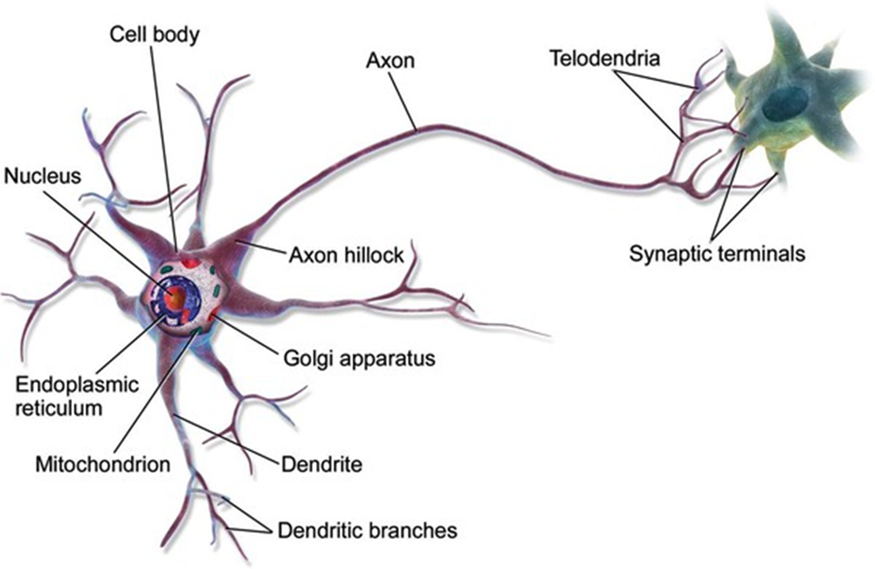
\includegraphics[width=\textwidth,height=0.7\textheight,keepaspectratio]{../machineLearningWeb/Figures/CH10/Hinh_10-1.png}
            \vspace{0.1cm}
            \captionof{figure}{Hình 10-1: Cấu trúc của Nơ-ron sinh học}
        \end{column}
    \end{columns}
\end{frame}

% 6
\begin{frame}{1.3 Từ Sinh học đến Mô hình Nhân tạo}
    \begin{itemize}
        \item Mô hình nơ-ron nhân tạo đầu tiên (Mô hình McCulloch-Pitts) cực kỳ đơn giản.
        \item Một nơ-ron nhân tạo có một hoặc nhiều đầu vào (nhị phân), và một đầu ra.
        \item Nơ-ron kích hoạt (phát tín hiệu 1) khi một lượng đủ lớn các đầu vào của nó kích hoạt.
        \item Mặc dù đơn giản, nhưng khi kết nối chúng thành một mạng lưới, ta có thể tính toán bất kỳ biểu thức logic nào.
    \end{itemize}
\end{frame}

% 7
\begin{frame}{1.4 Các Phép toán Logic với Nơ-ron}
    \begin{columns}
        \begin{column}{0.45\textwidth}
            \begin{itemize}
                \item Mạng (a): Hàm IDENTITY. 
                \item Mạng (b): Hàm AND (Chỉ sáng khi cả hai đều sáng).
                \item Mạng (c): Hàm OR (Sáng khi 1 trong 2 sáng).
                \item Mạng (d): Cổng logic phức tạp.
            \end{itemize}
        \end{column}
        \begin{column}{0.55\textwidth}
            \centering
            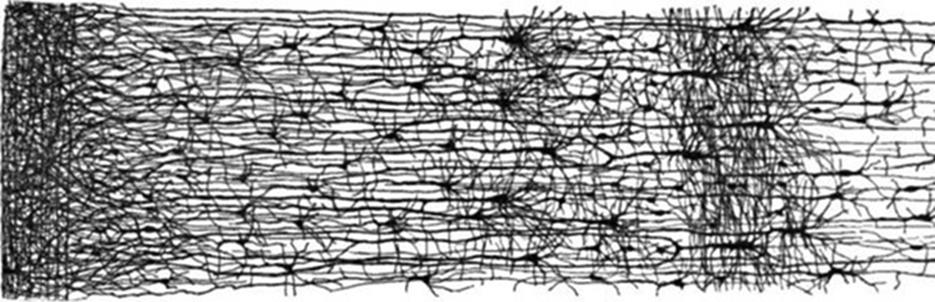
\includegraphics[width=\textwidth,height=0.7\textheight,keepaspectratio]{../machineLearningWeb/Figures/CH10/Hinh_10-2.jpg}
            \vspace{0.1cm}
            \captionof{figure}{Hình 10-2: Các phép tính logic đơn giản}
        \end{column}
    \end{columns}
\end{frame}

%==================================================================
\section{2. Perceptron}
%==================================================================

% 8
\begin{frame}{2.1 Khái niệm Perceptron}
    \begin{itemize}
        \item Perceptron do Frank Rosenblatt phát minh năm 1957.
        \item Nó dựa trên một loại nơ-ron nhân tạo gọi là \textbf{TLU (Threshold Logic Unit)} hay \textbf{LTU (Linear Threshold Unit)}.
        \item Thay vì nhị phân, TLU nhận đầu vào là các con số.
        \item Mỗi kết nối đầu vào được gán một trọng số (Weight) $w$.
    \end{itemize}
\end{frame}

% 9
\begin{frame}{2.2 Hoạt động của TLU (Threshold Logic Unit)}
    \begin{columns}
        \begin{column}{0.4\textwidth}
            \begin{itemize}
                \item Tính tổng trọng số: $z = w_1 x_1 + w_2 x_2 + ... + b = \mathbf{w}^T \mathbf{x} + b$.
                \item Sau đó áp dụng hàm bước (Step function) vào $z$: $h_{\mathbf{w}}(\mathbf{x}) = step(z)$.
                \item Hàm bước thường dùng là hàm \textbf{Heaviside} (Trả về 1 nếu $z \ge 0$, ngược lại 0).
            \end{itemize}
        \end{column}
        \begin{column}{0.6\textwidth}
            \centering
            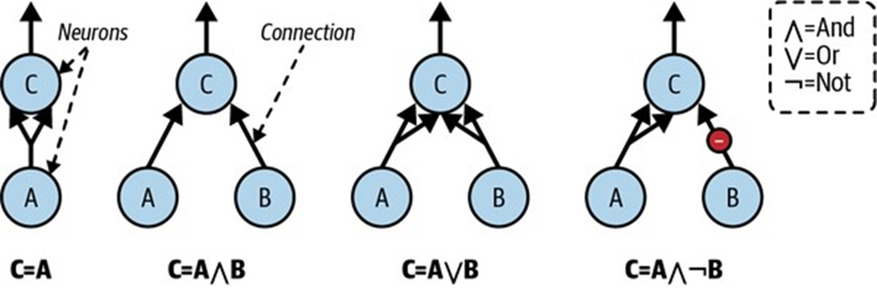
\includegraphics[width=\textwidth,height=0.7\textheight,keepaspectratio]{../machineLearningWeb/Figures/CH10/Hinh_10-3.png}
            \vspace{0.1cm}
            \captionof{figure}{Hình 10-3: Threshold Logic Unit (TLU)}
        \end{column}
    \end{columns}
\end{frame}

% 10
\begin{frame}{2.3 Kiến trúc Mạng Perceptron}
    \begin{columns}
        \begin{column}{0.45\textwidth}
            \begin{itemize}
                \item Perceptron bao gồm một lớp các TLU kết nối với tất cả các đầu vào (Lớp dày đặc - Dense Layer).
                \item Hình bên cho thấy một mạng Perceptron với 2 đầu vào, 1 nơ-ron bias, và 3 nơ-ron đầu ra.
                \item Mạng này có thể phân loại đa nhãn (Multi-output classification).
            \end{itemize}
        \end{column}
        \begin{column}{0.55\textwidth}
            \centering
            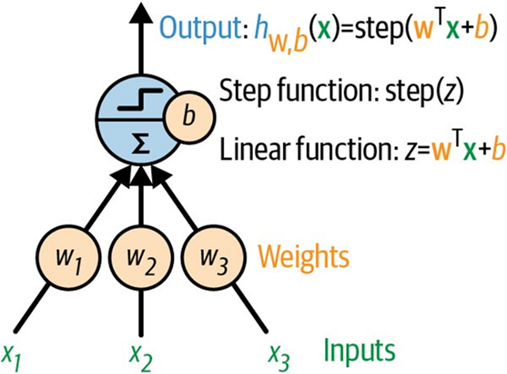
\includegraphics[width=\textwidth,height=0.7\textheight,keepaspectratio]{../machineLearningWeb/Figures/CH10/Hinh_10-4.png}
            \vspace{0.1cm}
            \captionof{figure}{Hình 10-4: Mạng Perceptron}
        \end{column}
    \end{columns}
\end{frame}

% 11
\begin{frame}{2.4 Điểm yếu của Perceptron: Bài toán XOR}
    \begin{columns}
        \begin{column}{0.4\textwidth}
            \begin{itemize}
                \item Năm 1969, Minsky và Papert chứng minh Perceptron có nhược điểm nghiêm trọng.
                \item Chúng là các bộ phân loại tuyến tính, do đó không thể giải bài toán \textbf{XOR (Exclusive OR)}.
                \item Hình bên cho thấy bài toán XOR không thể bị cắt đôi bằng một đường thẳng.
            \end{itemize}
        \end{column}
        \begin{column}{0.6\textwidth}
            \centering
            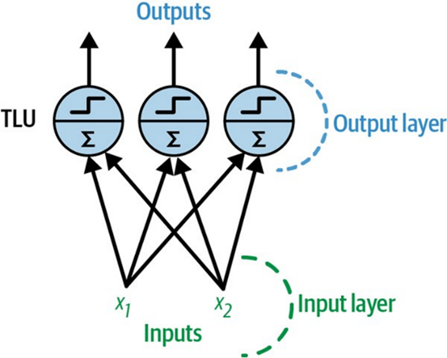
\includegraphics[width=\textwidth,height=0.7\textheight,keepaspectratio]{../machineLearningWeb/Figures/CH10/Hinh_10-5.png}
            \vspace{0.1cm}
            \captionof{figure}{Hình 10-5: Điểm yếu giải quyết XOR}
        \end{column}
    \end{columns}
\end{frame}

%==================================================================
\section{3. Mạng Perceptron Đa lớp (MLP)}
%==================================================================

% 12
\begin{frame}{3.1 Mạng Perceptron Đa Lớp (MLP)}
    \begin{itemize}
        \item Khắc phục sự cố XOR bằng cách xếp chồng nhiều Perceptron lên nhau $\rightarrow$ \textbf{Multi-Layer Perceptron (MLP)}.
        \item Kiến trúc MLP bao gồm:
        \begin{enumerate}
            \item Lớp Đầu vào (Input Layer).
            \item Một hoặc nhiều Lớp Ẩn (Hidden Layers).
            \item Lớp Đầu ra (Output Layer).
        \end{enumerate}
        \item Bất kỳ mạng nơ-ron nào có từ 2 lớp ẩn trở lên được gọi là \textbf{Học Sâu (Deep Learning)}.
    \end{itemize}
\end{frame}

% 13
\begin{frame}{3.2 Kiến trúc MLP}
    \begin{columns}
        \begin{column}{0.4\textwidth}
            \begin{itemize}
                \item Mỗi lớp (ngoại trừ lớp ra) thường bao gồm một nơ-ron bias.
                \item Các nơ-ron ở một lớp được kết nối đầy đủ (Fully Connected) đến mọi nơ-ron ở lớp tiếp theo.
                \item Dữ liệu luôi trôi theo 1 chiều (từ trái qua phải), gọi là Mạng truyền thẳng (Feedforward Neural Network - FNN).
            \end{itemize}
        \end{column}
        \begin{column}{0.6\textwidth}
            \centering
            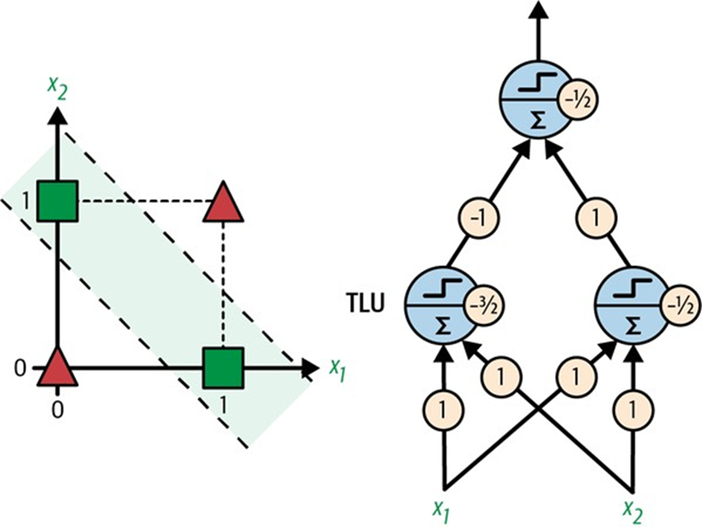
\includegraphics[width=\textwidth,height=0.7\textheight,keepaspectratio]{../machineLearningWeb/Figures/CH10/Hinh_10-6.png}
            \vspace{0.1cm}
            \captionof{figure}{Hình 10-6: Kiến trúc Mạng Perceptron Đa lớp}
        \end{column}
    \end{columns}
\end{frame}

% 14
\begin{frame}{3.3 Thuật toán Lan truyền ngược (Backpropagation)}
    \begin{itemize}
        \item Năm 1986, Rumelhart, Hinton và Williams công bố bài báo giới thiệu thuật toán \textbf{Backpropagation} kết hợp \textbf{Gradient Descent}.
        \item Backprop là linh hồn của Deep Learning ngày nay.
        \item Quá trình hoạt động:
        \begin{enumerate}
            \item Lan truyền tiến (Forward Pass): Tính kết quả dự đoán.
            \item Tính toán Lỗi (Compute Error): So sánh kết quả với thực tế.
            \item Lan truyền ngược (Backward Pass): Tính đạo hàm (Gradient) của lỗi với từng trọng số (Sử dụng Chain Rule / Autodiff).
            \item Cập nhật Trọng số (Gradient Descent Step).
        \end{enumerate}
    \end{itemize}
\end{frame}

% 15
\begin{frame}{3.4 Tại sao lại cần Hàm Kích hoạt (Activation Functions)?}
    \begin{itemize}
        \item Để Backprop hoạt động, người ta thay hàm bước (Step function) bằng các hàm liên tục có đạo hàm khác không.
        \item Nếu chỉ cộng dồn tuyến tính, mạng nơ-ron 100 lớp cũng chỉ ngang bằng mạng 1 lớp (Vì hàm tuyến tính tổ hợp lại vẫn là tuyến tính).
        \item Hàm kích hoạt mang tính \textbf{phi tuyến tính (Non-linearity)}, giúp mạng học được các hàm phức tạp.
    \end{itemize}
\end{frame}

% 16
\begin{frame}{3.5 Các Hàm Kích Hoạt Phổ Biến}
    \begin{columns}
        \begin{column}{0.35\textwidth}
            \begin{itemize}
                \item \textbf{Sigmoid:} Ép đầu ra về khoảng [0, 1]. Dùng cho phân loại nhị phân.
                \item \textbf{Tanh:} Ép về [-1, 1], có tâm tại 0.
                \item \textbf{ReLU:} Bằng 0 nếu âm, giữ nguyên nếu dương. Nhanh, đạo hàm tốt, là mặc định cho các lớp ẩn hiện nay.
            \end{itemize}
        \end{column}
        \begin{column}{0.65\textwidth}
            \centering
            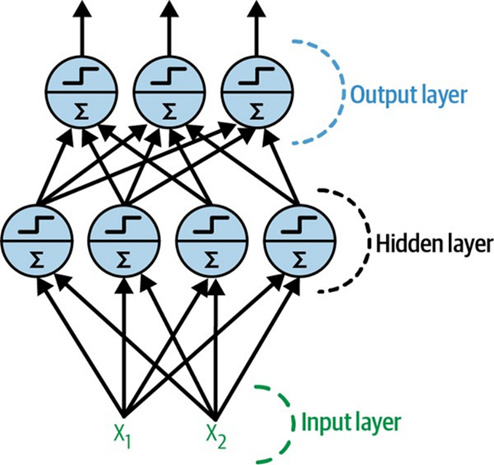
\includegraphics[width=\textwidth,height=0.7\textheight,keepaspectratio]{../machineLearningWeb/Figures/CH10/Hinh_10-7.png}
            \vspace{0.1cm}
            \captionof{figure}{Hình 10-7: Bảng các Hàm kích hoạt (Activation Functions)}
        \end{column}
    \end{columns}
\end{frame}

%==================================================================
\section{4. MLP Hồi quy \& Phân loại}
%==================================================================

% 17
\begin{frame}{4.1 MLP Hồi quy (Regression MLP)}
    \begin{itemize}
        \item Hồi quy dự đoán một giá trị liên tục (Ví dụ: Giá nhà).
        \item Lớp đầu ra chỉ cần \textbf{1 nơ-ron duy nhất} (Không dùng hàm kích hoạt).
        \item Nếu dự đoán giá trị phải luôn dương, dùng hàm kích hoạt \textbf{ReLU} hoặc \textbf{Softplus} ở đầu ra.
        \item Hàm mất mát (Loss function): \textbf{MSE (Mean Squared Error)} hoặc \textbf{MAE (Mean Absolute Error)}.
    \end{itemize}
\end{frame}

% 18
\begin{frame}{4.2 Cấu hình chuẩn cho MLP Hồi quy}
    \begin{table}[]
        \centering
        \resizebox{\textwidth}{!}{
        \begin{tabular}{ll}
        \toprule
        \textbf{Hyperparameter} & \textbf{Typical Value} \\
        \midrule
        Nơ-ron đầu vào (Input) & Một nơ-ron cho mỗi đặc trưng (Feature). \\
        Số lớp ẩn (Hidden Layers) & Tùy thuộc bài toán, thường từ 1 đến 5. \\
        Nơ-ron mỗi lớp ẩn & Thường từ 10 đến 100. \\
        Nơ-ron đầu ra (Output) & 1 (Nếu tiên đoán 1 giá trị), N (Nếu tiên đoán N chiều). \\
        Hàm kích hoạt (Lớp ẩn) & ReLU (Hoặc SELU, Mish). \\
        Hàm kích hoạt (Đầu ra) & None (Liên tục), ReLU (Dương), Sigmoid (Khoảng 0-1). \\
        Hàm mất mát (Loss) & MSE, MAE, hoặc Huber Loss. \\
        \bottomrule
        \end{tabular}}
        \caption{Hình 10-8: Kiến trúc MLP Hồi quy chuẩn}
    \end{table}
\end{frame}

% 19
\begin{frame}{4.3 MLP Phân loại (Classification MLP)}
    \begin{itemize}
        \item \textbf{Phân loại nhị phân (Binary):} Dùng 1 nơ-ron đầu ra với hàm \textbf{Sigmoid}. (Xác suất từ 0 đến 1). Loss: Binary Crossentropy.
        \item \textbf{Phân loại đa nhãn (Multilabel):} Vd nhận dạng email vừa là spam vừa là urgent. Dùng N nơ-ron đầu ra, mỗi nơ-ron có hàm \textbf{Sigmoid}. Loss: Binary Crossentropy.
        \item \textbf{Phân loại đa lớp (Multiclass):} Vd nhận diện MNIST (Từ 0 đến 9). Dùng N nơ-ron đầu ra với hàm \textbf{Softmax}. Loss: Categorical Crossentropy.
    \end{itemize}
\end{frame}

% 20
\begin{frame}{4.4 Cấu hình chuẩn cho MLP Phân loại}
    \begin{table}[]
        \centering
        \resizebox{\textwidth}{!}{
        \begin{tabular}{llll}
        \toprule
        \textbf{Hyperparameter} & \textbf{Binary} & \textbf{Multilabel} & \textbf{Multiclass} \\
        \midrule
        Input \& Hidden & \multicolumn{3}{c}{Giống như Hồi quy (1-5 lớp, ReLU)} \\
        Output Neurons & 1 & 1 cho mỗi nhãn & 1 cho mỗi lớp (Tổng cộng N) \\
        Output Activation & \textbf{Sigmoid} & \textbf{Sigmoid} & \textbf{Softmax} \\
        Loss Function & Binary Crossentropy & Binary Crossentropy & Categorical Crossentropy \\
        \bottomrule
        \end{tabular}}
        \caption{Hình 10-9: Kiến trúc MLP Phân loại chuẩn}
    \end{table}
\end{frame}


%==================================================================
\section{5. Triển khai MLP với Keras}
%==================================================================

% 21
\begin{frame}{5.1 TensorFlow và Keras}
    \begin{itemize}
        \item \textbf{TensorFlow:} Thư viện mã nguồn mở cho Học sâu của Google. Xử lý đồ thị tính toán mạnh mẽ trên CPU, GPU, TPU.
        \item \textbf{Keras:} API bậc cao (High-level API) của TensorFlow. Cực kỳ thân thiện với người dùng, dễ học, nhưng đủ linh hoạt để tuỳ chỉnh mô hình chuyên sâu.
        \item Hướng dẫn sau sử dụng bộ dữ liệu \textbf{Fashion MNIST} (Nhận diện ảnh 28x28 của các mặt hàng quần áo thời trang).
    \end{itemize}
\end{frame}

% 22
\begin{frame}[fragile]{5.2 Sequential API: Xây dựng mô hình}
    \begin{itemize}
        \item Keras \texttt{Sequential} API tạo mô hình bằng cách xếp chồng các lớp (Layer) tuần tự.
    \end{itemize}
\begin{lstlisting}[language=Python]
import tensorflow as tf
from tensorflow import keras

model = keras.models.Sequential([
    keras.layers.Flatten(input_shape=[28, 28]),
    keras.layers.Dense(300, activation="relu"),
    keras.layers.Dense(100, activation="relu"),
    keras.layers.Dense(10, activation="softmax")
])
model.summary() # Xem tom tat cau truc mo hinh
\end{lstlisting}
\end{frame}

% 23
\begin{frame}{5.3 Giải thích Mô hình Sequential}
    \begin{itemize}
        \item \texttt{Flatten}: Lớp chuyển đổi ảnh ma trận 2D (28x28) thành mảng 1D (784). (Không có trọng số).
        \item \texttt{Dense(300)}: Lớp ẩn đầu tiên với 300 nơ-ron kết nối đầy đủ. Số tham số = 784 x 300 + 300 (bias) = 235,500.
        \item \texttt{Dense(100)}: Lớp ẩn thứ hai với 100 nơ-ron. (30,100 tham số).
        \item \texttt{Dense(10)}: Lớp đầu ra với 10 nơ-ron (cho 10 lớp mặt hàng). Dùng Softmax để xuất ra xác suất tổng bằng 1.
    \end{itemize}
\end{frame}

% 24
\begin{frame}[fragile]{5.4 Biên dịch (Compile) và Huấn luyện (Fit)}
\begin{lstlisting}[language=Python]
# Buoc 1: Compile - Khai bao Loss va Optimizer
model.compile(loss="sparse_categorical_crossentropy",
              optimizer="sgd",
              metrics=["accuracy"])

# Buoc 2: Fit - Huan luyen mo hinh (Lan truyen nguooc)
history = model.fit(X_train, y_train, epochs=30,
                    validation_data=(X_valid, y_valid))
\end{lstlisting}
    \begin{itemize}
        \item \texttt{sparse\_categorical\_crossentropy}: Dùng vì nhãn Y là các số nguyên rải rác (0-9).
        \item \texttt{sgd}: Stochastic Gradient Descent.
        \item \texttt{epochs=30}: Huấn luyện duyệt qua toàn bộ tập dữ liệu 30 lần.
    \end{itemize}
\end{frame}

% 25
\begin{frame}{5.5 Đường cong Học tập (Learning Curves)}
    \begin{columns}
        \begin{column}{0.4\textwidth}
            \begin{itemize}
                \item Object \texttt{history} chứa dữ liệu loss và accuracy của train/valid sau mỗi epoch.
                \item Nhìn vào biểu đồ, Loss liên tục giảm dần (tốt).
                \item Accuracy liên tục tăng (tốt).
                \item Nếu Validation Loss đi ngang hoặc tăng lên, mô hình đang bị \textbf{Overfitting}.
            \end{itemize}
        \end{column}
        \begin{column}{0.6\textwidth}
            \centering
            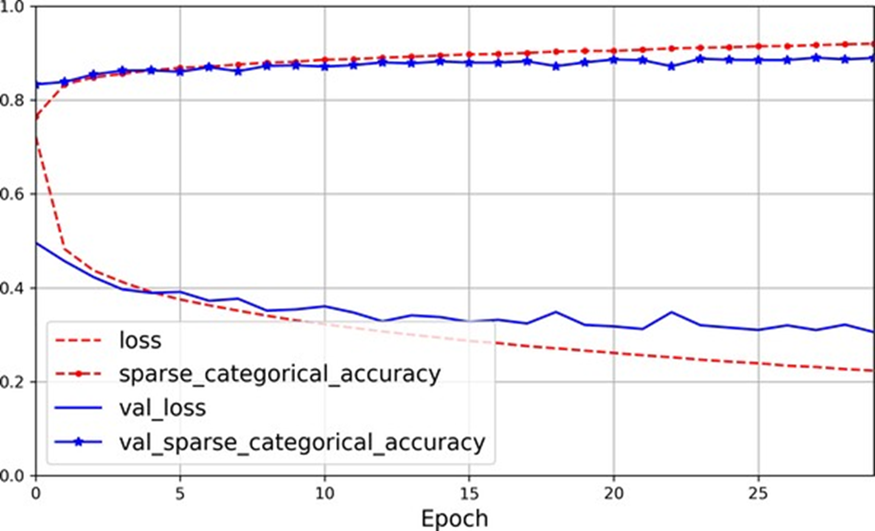
\includegraphics[width=\textwidth,height=0.65\textheight,keepaspectratio]{../machineLearningWeb/Figures/CH10/Hinh_10-11.png}
            \vspace{0.1cm}
            \captionof{figure}{Hình 10-11: Đồ thị Loss và Accuracy theo số vòng lặp (Epoch)}
        \end{column}
    \end{columns}
\end{frame}


%==================================================================
\section{6. Functional API \& Subclassing API}
%==================================================================

% 26
\begin{frame}{6.1 Vượt giới hạn với Functional API}
    \begin{itemize}
        \item Mô hình tuần tự (Sequential) rất phổ biến, nhưng đôi khi ta cần cấu trúc phi tuần tự.
        \item Ví dụ: \textbf{Wide \& Deep Neural Network}.
        \item Kiến trúc này nối trực tiếp lớp Đầu vào (Input) với lớp Đầu ra (Output) song song cùng với Lớp ẩn sâu.
        \item Cho phép mạng học được cả \textbf{Mẫu sâu (Deep patterns)} lẫn \textbf{Quy luật nông (Simple rules)}.
    \end{itemize}
\end{frame}

% 27
\begin{frame}{6.2 Kiến trúc Wide \& Deep}
    \begin{columns}
        \begin{column}{0.4\textwidth}
            \begin{itemize}
                \item Các mô hình MLP thông thường ép mọi dữ liệu chảy qua một chuỗi các lớp ẩn, khiến các quy luật đơn giản ban đầu có thể bị biến dạng hoặc "quên" mất.
                \item Kiến trúc Wide \& Deep chia nhánh để bảo toàn các đặc trưng đầu vào gốc.
            \end{itemize}
        \end{column}
        \begin{column}{0.6\textwidth}
            \centering
            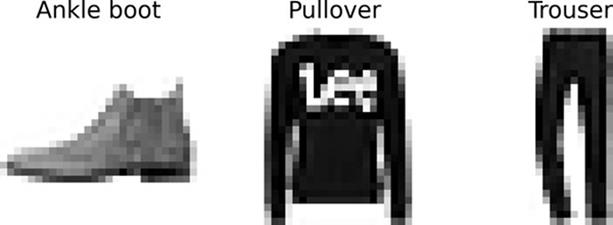
\includegraphics[width=\textwidth,height=0.7\textheight,keepaspectratio]{../machineLearningWeb/Figures/CH10/Hinh_10-12.jpg}
            \vspace{0.1cm}
            \captionof{figure}{Hình 10-12: Mạng Nơ-ron Rộng và Sâu (Wide \& Deep)}
        \end{column}
    \end{columns}
\end{frame}

% 28
\begin{frame}[fragile]{6.3 Code: Functional API}
\begin{lstlisting}[language=Python]
input_ = keras.layers.Input(shape=X_train.shape[1:])
hidden1 = keras.layers.Dense(30, activation="relu")(input_)
hidden2 = keras.layers.Dense(30, activation="relu")(hidden1)

# Ghep noi (Concatenate) duong "Wide" va "Deep"
concat = keras.layers.Concatenate()([input_, hidden2])

output = keras.layers.Dense(1)(concat)
model = keras.models.Model(inputs=[input_], outputs=[output])
\end{lstlisting}
    \begin{itemize}
        \item Trong Functional API, ta phải gọi từng lớp như một hàm và truyền input vào.
        \item Cuối cùng, bọc tất cả lại trong \texttt{keras.models.Model}.
    \end{itemize}
\end{frame}

% 29
\begin{frame}{6.4 Functional API: Nhiều luồng dữ liệu (Multiple Inputs)}
    \begin{columns}
        \begin{column}{0.4\textwidth}
            \begin{itemize}
                \item Sẽ ra sao nếu ta muốn gửi một nhóm đặc trưng vào "Đường rộng", và một nhóm đặc trưng khác vào "Đường sâu"?
                \item Keras Functional API có thể tạo nhiều luồng Input.
                \item Lúc gọi hàm \texttt{fit()}, ta sẽ truyền \texttt{(X\_train\_A, X\_train\_B)}.
            \end{itemize}
        \end{column}
        \begin{column}{0.6\textwidth}
            \centering
            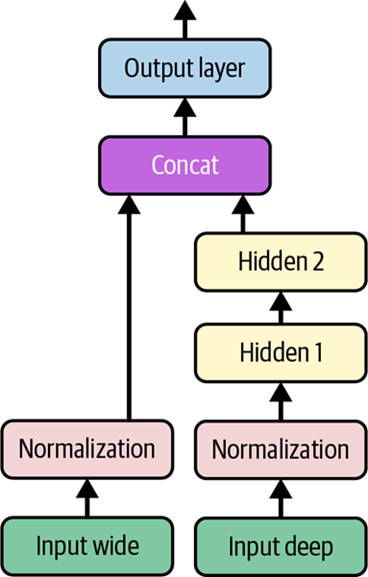
\includegraphics[width=\textwidth,height=0.7\textheight,keepaspectratio]{../machineLearningWeb/Figures/CH10/Hinh_10-14.png}
            \vspace{0.1cm}
            \captionof{figure}{Hình 10-14: Xử lý nhiều luồng đầu vào}
        \end{column}
    \end{columns}
\end{frame}

% 30
\begin{frame}{6.5 Functional API: Nhiều đầu ra (Multiple Outputs)}
    \begin{columns}
        \begin{column}{0.4\textwidth}
            \begin{itemize}
                \item Tương tự, một mạng cũng có thể có nhiều đầu ra.
                \item Ví dụ: Phát hiện vật thể trên ảnh (1 Output là Phân loại vật, 1 Output khác là Tọa độ đóng khung vật).
                \item Mỗi Output sẽ có một \texttt{loss} riêng biệt. Keras tính toán theo tổng các loss có hệ số nhân.
            \end{itemize}
        \end{column}
        \begin{column}{0.6\textwidth}
            \centering
            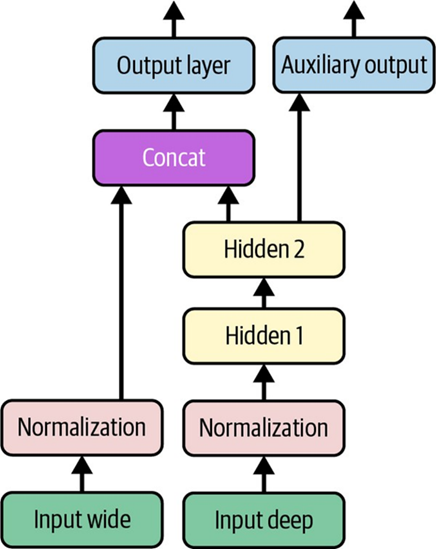
\includegraphics[width=\textwidth,height=0.7\textheight,keepaspectratio]{../machineLearningWeb/Figures/CH10/Hinh_10-15.png}
            \vspace{0.1cm}
            \captionof{figure}{Hình 10-15: Mạng có nhiều đầu ra}
        \end{column}
    \end{columns}
\end{frame}

% 31
\begin{frame}[fragile]{6.6 Subclassing API (Lập trình Hướng đối tượng)}
    \begin{itemize}
        \item Cả Sequential và Functional API đều là "Tuyên bố" (Declarative). Nghĩa là mô hình là đồ thị tĩnh.
        \item Nếu bạn cần một mô hình với kiến trúc "Động", có vòng lặp, có \texttt{if/else} hoạt động linh hoạt, hãy dùng \textbf{Subclassing API}.
    \end{itemize}
\begin{lstlisting}[language=Python]
class WideAndDeepModel(keras.models.Model):
    def __init__(self, units=30, activation="relu", **kwargs):
        super().__init__(**kwargs)
        self.hidden1 = keras.layers.Dense(units, activation=activation)
        self.hidden2 = keras.layers.Dense(units, activation=activation)
        self.main_output = keras.layers.Dense(1)
        
    def call(self, inputs): # Dinh nghia cach truyen tien tai day
        hidden1 = self.hidden1(inputs)
        hidden2 = self.hidden2(hidden1)
        concat = keras.layers.concatenate([inputs, hidden2])
        return self.main_output(concat)
\end{lstlisting}
\end{frame}

%==================================================================
\section{7. Lưu Mô hình \& Kỹ thuật nâng cao}
%==================================================================

% 32
\begin{frame}[fragile]{7.1 Lưu và Khôi phục Mô hình}
    \begin{itemize}
        \item Quá trình huấn luyện Mạng Nơ-ron tốn rất nhiều thời gian (Có thể vài ngày). Bạn cần lưu lại!
        \item Keras lưu mô hình theo định dạng HDF5 (.h5). Nó chứa toàn bộ Trọng số, Cấu trúc, Optimizer.
    \end{itemize}
\begin{lstlisting}[language=Python]
# Luu model
model.save("my_keras_model.h5")

# Phuc hoi model
model = keras.models.load_model("my_keras_model.h5")
\end{lstlisting}
\end{frame}

% 33
\begin{frame}[fragile]{7.2 Callbacks: Trợ lý huấn luyện}
    \begin{itemize}
        \item Keras cho phép gọi các hàm \textbf{Callback} ở mỗi cuối Epoch hoặc cuối Batch.
        \item \textbf{ModelCheckpoint}: Tự động lưu mô hình mỗi khi nó "Đạt điểm cao nhất" trên tập Validation (Tránh mất mô hình tốt nhất nếu bị sập nguồn).
    \end{itemize}
\begin{lstlisting}[language=Python]
checkpoint_cb = keras.callbacks.ModelCheckpoint("my_best_model.h5", 
                                                save_best_only=True)
history = model.fit(X_train, y_train, epochs=10, 
                    validation_data=(X_valid, y_valid),
                    callbacks=[checkpoint_cb])
\end{lstlisting}
\end{frame}

% 34
\begin{frame}[fragile]{7.3 Dừng sớm (Early Stopping)}
    \begin{itemize}
        \item Không ai biết cần đặt \texttt{epochs} bao nhiêu là vừa. Đặt lớn quá sẽ gây Overfitting.
        \item \textbf{EarlyStopping}: Tự động "Rút phích cắm" dừng huấn luyện nếu nhận thấy Loss trên tập Validation không còn cải thiện.
    \end{itemize}
\begin{lstlisting}[language=Python]
early_stopping_cb = keras.callbacks.EarlyStopping(patience=10,
                                                  restore_best_weights=True)
# patience=10 nghia la doi them 10 epoch xem co hy vong khong.
history = model.fit(X_train, y_train, epochs=1000, # Dat epoch 1000 cho thoai mai
                    validation_data=(X_valid, y_valid),
                    callbacks=[checkpoint_cb, early_stopping_cb])
\end{lstlisting}
\end{frame}

% 35
\begin{frame}{7.4 TensorBoard: Công cụ Giám sát tối thượng}
    \begin{itemize}
        \item TensorFlow cung cấp \textbf{TensorBoard}, một giao diện đồ họa siêu cấp để theo dõi quá trình huấn luyện trực tiếp.
        \item Nó vẽ đồ thị Loss, Accuracy theo thời gian thực.
        \item Hiển thị sơ đồ đồ thị kết nối Lớp (Graph).
        \item Cực kỳ hữu ích để gỡ lỗi các mạng khổng lồ.
        \item Ghi log bằng cách truyền \texttt{keras.callbacks.TensorBoard(log\_dir="logs")} vào \texttt{callbacks}.
    \end{itemize}
\end{frame}


%==================================================================
\section{8. Tinh chỉnh Siêu Tham số}
%==================================================================

% 36
\begin{frame}{8.1 Tinh chỉnh Siêu Tham số (Hyperparameters)}
    \begin{itemize}
        \item Mạng Nơ-ron có độ linh hoạt tuyệt đối. Đồng nghĩa với việc có hàng tá thông số cần tinh chỉnh!
        \item Làm sao để biết mạng nên có 2 lớp hay 100 lớp ẩn?
        \item Phương pháp cơ bản: Sử dụng \texttt{GridSearchCV} hoặc \texttt{RandomizedSearchCV}.
        \item Tuy nhiên, với Mạng Sâu, \texttt{RandomizedSearch} hiệu quả hơn nhiều. Bạn cũng có thể dùng công cụ \textbf{Keras Tuner}.
    \end{itemize}
\end{frame}

% 37
\begin{frame}{8.2 Số lượng Lớp Ẩn (Hidden Layers)}
    \begin{itemize}
        \item Mạng có 1 lớp ẩn với cấu trúc rộng theo lý thuyết có thể xấp xỉ bất kỳ hàm nào. Nhưng rất tốn tham số!
        \item \textbf{Mạng Sâu (Nhiều lớp ẩn):} Có hiệu suất tham số lớn hơn (parameter efficiency). Nó học cách phân cấp dữ liệu.
        \item Ví dụ nhận diện mặt: Lớp 1 học vẽ đoạn thẳng, lớp 2 vẽ thành mắt/mũi/miệng, lớp 3 gộp thành khuôn mặt.
        \item Kinh nghiệm: Hãy bắt đầu với 1 hoặc 2 lớp ẩn (Nó sẽ hoạt động tốt cho đa số bài toán). Đối với ảnh phức tạp, cần hàng chục lớp.
    \end{itemize}
\end{frame}

% 38
\begin{frame}{8.3 Số lượng Nơ-ron trên mỗi Lớp Ẩn}
    \begin{itemize}
        \item Cách thiết kế cổ điển (Hình phễu): Lớp đầu có nhiều nơ-ron (Vd: 300), lớp tiếp theo giảm dần (100), rồi (50)... nhằm tinh lọc dữ liệu.
        \item Tuy nhiên, nghiên cứu chỉ ra rằng \textbf{đặt số nơ-ron bằng nhau} ở mọi lớp ẩn (ví dụ: tất cả 150) cho ra kết quả tương tự, thậm chí tốt hơn, mà lại giảm bớt số tham số bạn phải nghĩ cách cấu hình.
        \item Mẹo vặt chiến thuật: Hãy chọn mô hình có số lớp và số nơ-ron "thừa thãi" nhiều hơn mức cần thiết, sau đó sử dụng \textbf{Early Stopping} và \textbf{Dropout} để ngăn nó Overfitting.
    \end{itemize}
\end{frame}

% 39
\begin{frame}{8.4 Tốc độ học (Learning Rate)}
    \begin{itemize}
        \item Tốc độ học (\texttt{lr}) là siêu tham số \textbf{QUAN TRỌNG NHẤT}. Nếu chỉ có thời gian tinh chỉnh 1 tham số, hãy tinh chỉnh cái này!
        \item Nếu \texttt{lr} quá lớn: Mạng sẽ nhảy qua lại không thể hội tụ (Diverge).
        \item Nếu \texttt{lr} quá nhỏ: Mất rất nhiều ngày tháng để huấn luyện.
        \item Giá trị khởi điểm kinh điển: $10^{-3}$ hoặc $10^{-4}$.
    \end{itemize}
\end{frame}

% 40
\begin{frame}{8.5 Kích thước Lô (Batch Size) \& Optimizer}
    \begin{itemize}
        \item \textbf{Batch Size:} Thường từ 32 đến 128. Batch Size quá to sẽ huấn luyện nhanh nhờ GPU nhưng có nguy cơ rơi vào tối ưu cục bộ. Batch Size nhỏ tốn CPU, tốn thời gian nhưng mang tính "nhảy múa" cao, dễ thoát hố sâu cục bộ.
        \item \textbf{Optimizer:} Thuật toán \textbf{Adam} Optimizer (Sẽ học ở chương 11) được chứng minh tốt hơn nhiều so với \textbf{SGD} cổ điển và đang được dùng mặc định ở hầu hết bài toán Học sâu.
    \end{itemize}
\end{frame}

% 41
\begin{frame}
    \centering
    \Huge \textbf{HỎI \& ĐÁP}
\end{frame}

\end{document}
